\chapter{Probleme und Formale Sprachen}\label{einleitung}
%\section{Warum theoretische Informatik?}
Warum lohnt sich die Beschäftigung mit theoretischer Informatik?
Die kurze Antwort: Sie liefert einen wesentlichen Teil des Handwerkszeugs,
um die Potentiale und Grenzen der technischen Informationsverarbeitung zu verstehen.
Die lange Antwort soll dieses Skript geben.

Die Nützlichkeit eines Werkzeugs leuchtet dann ein,
wenn es hilft Probleme zu lösen.
Daher ist der Problembegriff im Mittelpunkt dieses Skripts.
Was also ist ein Problem im Sinne der theoretischen Informatik?

\section{Probleme}

Alltägliche IT-Aufgaben werden oft als Userstories dokumentiert.
Eine Userstory wird in der agilen Softwareentwicklung genutzt um Anforderungen zu spezifizieren.
Eine Userstory trifft man typischerweise in diesem Format an:
''Als \textless Rolle\textgreater\ möchte ich \textless Feature\textgreater,
um \textless Ziel\textgreater\ zu erreichen.''
Diese Beispiele für Userstories sollen uns im Skript begleiten:

\begin{itemize}
%TODO: Einkommentieren und Bearbeiten, wenn Kapitel geschrieben.
    \item \textbf{U\textsubscript{EVEN}}:
        Als Kommisionier:in möchte ich die Anzahl der geplanten Paletten pro LKW kennen, 
        um zu sehen, ob Platz für den Hubwagen bleibt.
     \item \textbf{U\textsubscript{SUPPLIERID}}:
        Als Einkaufsmanager:in möchte ich,
        dass nur valide Lieferanten-IDs gespeichert werden
        (beginnend mit einem ``S'', gefolgt von einer Zahl),
        um Fehler in der Datenbank zu vermeiden.
     \item \textbf{U\textsubscript{ARTICLESORT}}:
        Als Verantwortliche:r fürs Spiegel-Management
        will ich eine nach Verkaufszahlen sortierte Liste von Artikeln,
        um die Regalaufteilung daran auszurichten.
    \item \textbf{U\textsubscript{SORTIMENT}}:
        Als Einkaufsmanager:in möchte ich,
        dass das Sortiment in allen Filialien identisch ist,
        um alle anderen Prozesse darauf ausrichten zu können.
    \item \textbf{U\textsubscript{SUPPLYROUTE}}:
        Als Kommissionierer:in möchte ich,
        dass morgens die optimalen Routen für die LKWs in die 24 Filialen berechnet werden,
        um die Lieferzeit zu minimieren.
    \item \textbf{U\textsubscript{CLOUDHALT}}:
        Als Product Owner des Serverless-Computings möchte ich,
        dass nur terminierende Code-Snippets deployt werden,
        um die verfügbaren Ressourcen effizient zu nutzen.
%TODO: Einkommentieren und Bearbeiten, wenn nötig
%    \item \textbf{QUANTUMSEC}: Als Chief Security Officer möchte ich,
%        dass die firmen-interne Kommunikation quantensicher verschlüsselt wird,
%        um die Vertraulichkeit der Absprachen zu garantieren.
\end{itemize}

Erfahrene und kompetente IT-Fachkräfte identifizieren beim ersten Lesen einer Userstory
einen logischen ``Kern'',
also etwas das in unterschiedlichem Gewand öfters wiederkehrt.
Bis wir eine bessere Definition dieses Begriffs finden,
wollen wir diesen Kern als ``Problem'' bezeichnen,

Mit den Methoden der theoretischen Informatik ausgerüstet,
kann man einiges über die eben aufgeführten Userstories und deren zugrundeliegende Probleme sagen:
\begin{itemize}
    \item Mindestens eine Userstory ist leicht zu realisieren.
    \item Für mindestens eine Userstory kann man mit vertretbarem Aufwand nur suboptimale Lösungen finden.
    \item Mindestens eine Userstory ist nicht umsetzbar.
\end{itemize}
Um unnötige Arbeit zu vermeiden
und die besten der bekannten Lösungen zu implementieren,
ist natürlich von Interesse,
welche Userstory in welche dieser Kategorien fällt.
Dafür müssen wir die Ergebnisse und Werkzeuge
der theoretischen Informatik kennen und anwenden;
die Form der Userstory ist jedoch dafür nicht geeignet.

Damit wir das volle Potential der theoretischen Informatik schöpfen können,
müssen wir zwei Schritte gehen:
Wir müssen von den Userstories \emph{abstrahieren}
und diese Abstraktion \emph{formalisieren}.
Die beiden folgenden Abschnitte zeigen anhand \textbf{U\textsubscript{EVEN}}
beispielhaft, was damit gemeint ist.
Dabei werden wir die ersten zentralen Begriffe dieses Skriptes einführen und diskutieren.

\section{Abstraktion}

\emph{Abstraktion} ist die ausschließliche Betrachtung der Aspekte eines Sachverhalts,
die für einen gegebenen Zweck wesentlich sind.
Die Abstraktion ist der Weg von einer sehr speziellen Aufgabenbeschreibung,
wie einer Userstory, zu einem abstrakten Problem,
dessen Lösung in vielen spezifischen Kontexten anwendbar wird.
Im besten Fall ist diese Lösung bereits implementiert, frei verfügbar
und daher leicht nachnutzbar.

Es gibt leider keinen einfachen, eindeutigen oder automatisierbaren Weg
durch Abstraktion von einer Userstory zu einem abstrakten Problem zu kommen.
Dafür sind intellektuelle Kreativität
und ein gutes Verständnis des vorliegenden Zwecks notwendig.
Ein möglicher Fehler ist zum Beispiel,
zu wenige Aspekte auszulassen,
so dass das abstrakte Problem nicht so einfach wie möglich ist.
Ebenso ist es ein Fehler, zu viele Aspekte auszulassen,
so dass das abstrakte Problem nicht so detailreich wie nötig ist,
um dem vorliegenden Zweck gerecht zu werden.
Unser vorliegender Zweck ist die Einteilung der Userstories anhand deren Lösbarkeit.
So könnte eine Abstraktion von \textbf{U\textsubscript{EVEN}} für diesen Zweck aussehen:
\begin{enumerate}
    \item \emph{Als Kommissionier:in
         möchte ich die Anzahl der geplanten Paletten pro LKW kennen,
         um zu sehen, ob Platz für den Hubwagen bleibt.
        } (ursprüngliche Userstory).
    \item \emph{Identifikation der Anzahl an Paletten, um verfügbaren Platz zu quantifzieren.}
        (die Kenntnis der tatsächlichen Anzahl und wofür der Platz gedacht ist,
        ist für unseren Zweck gleichgültig.)
    \item \emph{Ist die Anzahl an Paletten (un)gerade?}
        (Es ist z.B. egal,
        ob zwei, drei oder mehr Paletten pro LKW nebeneinander passen,
        Hauptsache es bleibt Platz.)
    \item \emph{Ist eine Zahl gerade?}
        (Es ist egal, ob wir dies für Paletten oder andere Objekte entscheiden.)
\end{enumerate}

Wie wir im Laufe des Skriptes sehen werden,
führt die letzte Formulierung zu der wesentlichen Vorstufe,
um die Methoden der theoretischen Informatik anzuwenden.\footnote{
Es ist natürlich möglich,
dass die gezeigten Schritte nicht das richtige Resultat für einen anderen Zweck liefern.
Für eine Kommissionierer:in mag die Anzahl noch aus anderen Gründen interessant sein,
z.B. um die Auslastung der LKWs zu bewerten und zu optimieren.
Oder es mag nicht gleichgültig sein, ob zwei, drei oder mehr Paletten nebeneinander passen.
Wie man Abstraktionen im Sinne der Softwareentwicklung einsetzen kann,
lehrt die Disziplin des Software Engineerings.}
Wir kommen so auf den Kern der Userstory \textbf{U\textsubscript{EVEN}},
den wir \textbf{I\textsubscript{EVEN}} nennen wollen:
\begin{itemize}
    \item \textbf{Gegeben:} Eine Zahl
    \item \textbf{Gesucht:} Ein Wahrheitswert, der anzeigt, ob die Zahl gerade ist.
\end{itemize}
Diese Form der Problemangabe (Gegeben/Gesucht) bezeichnen wir als \emph{informell}
(daher das I).
Dabei ist für die informelle Angabe wichtig,
sowohl den Typ des (potentiell komplexen) Eingabewerts (hier: eine Zahl),
als auch des (potentiell komplexen) Ausgabewerts (hier: ein Wahrheitswert) zu spezifizieren.
Von der informellen Angabe eines Problems kommen wir zu der Einsicht,
dass sich ein Problem auch als Funktion beschreiben lässt,
also als Zuordnung von den ``Eingabewerten'' im Gegeben-Teil
(also der Definitionsmenge),
zu den ``Ausgabewerten'' im Gesucht-Teil
(der Wertemenge).

Die Fähigkeit via Abstraktion von vielen Alltagsaufgaben zu informellen Problemen zu kommen,
macht kompetenten IT-Fachkräften das Leben leichter:
Die Lösungen für wiederkehrende Probleme können
in Libraries, Best Practices und Dokumentationen gefunden oder eben festgehalten werden.
So sind Schablonen parat,
um schnell und effizient zu guten Ergebnissen zu kommen.

Aber die theoretische Informatik spielt hierbei keine explizite Rolle.
Ihre Methoden sind formal,
daher reicht auch \textbf{I\textsubscript{EVEN}} noch nicht aus,
wir benötigen eine formalere Version des Problems,
die wir mit \textbf{EVEN} bezeichnen.
Warum sollten wir diesen zusätzlichen Schritt gehen?
Wir können so über die Expertise erfahrener IT-Fachkräfte hinausgehen
und zweifelsfrei \emph{beweisen},
dass manche Probleme einfach, aufwändig oder unlösbar sind.\footnote{
    Eine etwas längere Antwort geben wir in \autoref{messenVsBeweisen}.
}
Wir stellen also daher drei Fragen exemplarisch für \textbf{EVEN},
die sich prinzipiell aber für alle Probleme ergeben:
\begin{enumerate}
    \item Welche Form muss \textbf{EVEN} haben, damit eine Maschine es lösen kann?\\
        In anderen Worten: Wie kann \textbf{EVEN} \emph{formalisiert} werden?
    \item Wie effizient kann eine Maschine \textbf{EVEN} lösen?\\
        In anderen Worten: Wie \emph{komplex} ist \textbf{EVEN}?
    \item Kann eine Maschine \textbf{EVEN} überhaupt lösen?\\
        In anderen Worten: Ist \textbf{EVEN} \emph{berechenbar}?
\end{enumerate}
Drei grundlegende Teildisziplinen der theoretischen Informatik
geben Antwort auf diese Art der Fragen:
\begin{enumerate}
    \item Die \textbf{Theorie der formalen Sprachen und Automaten}
    \item Die \textbf{Komplexitätstheorie}
    \item Die \textbf{Berechenbarkeitstheorie}
\end{enumerate}
Im Laufe des Skriptes werden wir
in grundlegende Ergebnisse dieser drei Teildisziplinen einführen,
ihre Wechselwirkung beschreiben
und Konsequenzen für die eingangs erwähnten Userstories ziehen.

\section{Formale Sprachen}\label{sec:formalisierung}

Damit wir die Werkzeuge der theoretischen Informatik anwenden können,
werden wir Probleme wie \textbf{EVEN} als formale Sprachen repräsentieren.
Dabei gehen wir in drei Schritten vor:
\begin{enumerate}
    \item Erklären, was eine formale Sprache ist (\autoref{subsec:formaleSprachen})
    \item Mit \textbf{I\textsubscript{EVEN}} beispielhaft zeigen,
        wie man ein informelles Problem in eine formale Sprache übersetzen kann
        (\autoref{subsec:problemeAlsFormaleSprachen})
    \item Diskutieren, warum formale Sprachen geeignete Repräsentationen für Probleme sind
        (\autoref{subsec:warumFormaleSprachen})
\end{enumerate}

\subsection{Formale Sprachen}\label{subsec:formaleSprachen}

Eine formale Sprache ist eine Menge von Worten,
die über einem Zeichenalphabet gebildet werden.
In diesem Abschnitt dröseln wir diesen Satz Schritt für Schritt auf:
Von Zeichen, über Worte, bis hin zu formalen Sprachen.

\subsubsection{Zeichen}

Eine Menge von Zeichen bezeichnen wir als \emph{Alphabet}, kurz: $\Sigma$.
Zum Beispiel wäre das kanonische Alphabet für die meisten IT-Systeme: $\Sigma = \{0,1\}$.\\

\noindent
Wir verwenden diese Variablen für Zeichen: $a,b,c$;
wenn wir diese Buchstaben verwenden und nichts anderes angeben,
gilt implizit: $a, b, c \in \Sigma$ für ein gegebenes $\Sigma$.\footnote{
Wenn $\Sigma$ nicht explizit angegeben oder aus dem Kontext herleitbar ist,
wird $\Sigma$ also auch als Variable für ein beliebiges Alphabet verwendet.}\\

\noindent
Die Grundoperation auf Zeichen ist die \emph{Konkatenation},
also die Verbindung von zwei Zeichen, z.B. $01$.
Wie bei der Multiplikation mit Variablen in der Mathematik üblich,
wird die Konketanation nicht explizit mit einem eigenen Zeichen repräsentiert.

\subsubsection{Worte}\label{words}
Das Ergebnis einer beliebig oft ausgeführten Konkatenation,
also eine Zeichenfolge,
bezeichnen wir als \emph{Wort}, zum Beispiel: $110$.
Worte selbst lassen sich ebenfalls konkatenieren,
Sei $v = 11$ und $w = 0$ dann ist $vw = 110$\\

\noindent
Die Menge aller Wörter,
die sich aus einem Alphabet bilden lassen,
bezeichnen wir als \emph{Kleenesche Hülle}, dargestellt als hochgestellter Stern: $\Sigma^*$.\\

\noindent
Wir verwenden diese Variablen für Worte:
$u, v, w, x, y, z$; wenn wir diese Buchstaben verwenden und nichts anderes angeben,
gilt implizit: $u, v, w, x, y, z \in \Sigma^*$.\\

\noindent
Die \emph{Länge} eines Wortes ist die Anzahl seiner Zeichen.
Formal benutzen wir die Betragsstriche um ein Wort, um seine
Länge zu bezeichnen. Wenn z.B. $w = 110$, dann gilt $|w| = 3$.\\

\noindent
Das Wort mit der Länge 0, also das Wort, dass aus null Zeichen besteht,
nennen wir das \emph{leere Wort}, kurz: $\epsilon$.
Es gilt $|\epsilon| = 0$.\\

\noindent
Für ein Wort $w$ mit $|w| \geq 1$ bezeichnet $w_i$ mit $0 \leq i < n$
genau das Zeichen in $w$ an der i-ten Stelle.
Sei zum Beispiel $w = 101$, dann ist $w_1 = 0$
(der Index ist null-basiert, wie bei Tupeln).\\

\noindent
Die \emph{Teilwortfunktion}
$tw: \Sigma^* \times \mathbb{N} \times \mathbb{N} \rightarrow \Sigma^*$
lässt sich definieren als das Teilwort $v$ beginnend an Index $i \in \mathbb{N}$
mit der Länge $|v| = l$ mit $l \in \mathbb{N}$:
$tw(w, i, l) = w_iw_{i+1}\ldots{}w_{i+l}$,
zum Beispiel ist $tw(1001, 1, 2) = 00$.\\

\noindent
Für die n-malige Wiederholung eines Zeichens oder Wortes führen wir den \emph{Wiederholungsoperator}
ein, eine hochgestellte Zahl $n \in \mathbb{N}$: $a^n$ oder $w^n$.
Z.B. $0^3 = 000$ und $(10)^2 = 1010$.
$a^0$ bzw. $w^0$ entspricht dabei $\epsilon$.\\

\noindent
Wollen wir angeben, dass ein Zeichen oder Wort beliebig oft (also auch 0-mal) wiederholt
wird, nutzen wir dafür einen hochgestellten Stern, den \emph{Kleene-Operator} $a^*$ oder $w^*$.
Mit dem Kleene-Operator bezeichnen wir immer eine unendliche Menge von Wörtern, z.B.:
$a^* = \{\epsilon, a, aa, aaa, aaaa, \dots\}$

\subsubsection{Formale Sprachen als Menge von Worten}

Bevor wir den Begriff der formalen Sprachen ordentlich einführen,
ist noch eine Warnung angebracht:
Während die Verwendung des Begriffs ''Zeichens''
noch recht intuitiv mit dem Begriff des Buchstaben zusammenfällt
(zumindest im deutschsprachigen Raum),
ist schon der formal eingeführte Wort-Begriff eher eine Zumutung für unsere Intuition:
Worte im Sinne des vorangegangenen Abschnitts sind einfach Zeichenfolgen,
egal ob sie aussprechbar oder im Kontext einer natürlichen Sprache
(wie Deutsch oder Englisch) einen Sinn ergeben.

%Man müsste also eigentlich das natursprachliche $Wort_N$ von dem formalen $Wort_F$ trennen,
%das wir oben eingeführt haben.
%Eine Crux aller formal arbeitenden Wissenschaften ist,
%dass die Menge an Zeichen und Begriffen begrenzt ist und daher Doppeldeutigkeiten auftreten.
%Wir müssen also durch Konventionen klären, welche Bedeutung wir einem Begriff geben wollen:
%Im Kontext dieses Skriptes bezeichnen wir mit dem Begriff Wort die Zeichenfolge, also $Wort_F$.
%Sollte dies nicht der Fall sein und der Kontext nicht ausreichen,
%um zwischen beiden Bedeutungen zu unterscheiden,
%werden wir die subskribierten Varianten verwenden.

Diese Überlegung trifft nicht nur auf Worte, sondern auch auf \emph{Sprachen} zu.
\textbf{Eine Sprache im Sinne der theoretischen Informatik ist einfach eine Menge von Worten.}
Z.B. ist $L = \{0, 1, 00, 01, 10, 11 \}$ die Sprache der Worte,
die aus einem oder zwei Binärzeichen bestehen.
Eine formale Sprache ist also als \emph{Menge} im Sinne der Mengenlehre aufzufassen,
nicht als Kommunikationsmedium mit einer eigenen Sprachgeschichte und Sprachgemeinschaft.\\

\noindent
Wir verwenden $L$ (ggf. mit unterschiedlichen Subskripten) als Variable für Sprachen;
wenn wir $L$ verwenden und nichts Anderslautendes angegeben ist,
gilt implizit $L \subseteq \Sigma^*$ für ein gegebenes $\Sigma$.\\

\noindent
Da Sprachen Mengen sind,
sind alle mengentheoretischen Operationen\footnote{
    Für die wesentlichen Operationen für dieses Skript siehe: \autoref{mengenlehre}}
auf Sprachen definiert,
z.B. bezeichnet $L_1 \cap L_2 = \{w | w \in L_1 \wedge w \in L_2\}$
die Schnittmenge zweier Sprachen, also alle Wörter,
die sowohl Element von $L_1$ als auch von $L_2$ sind.



\subsection{Probleme als formale Sprachen}\label{subsec:problemeAlsFormaleSprachen}

\subsubsection{Einstellige Wahrheitsfunktionen}
Wie bekommen wir nun ein Problem wie \textbf{I\textsubscript{EVEN}}
(Gegeben: Eine Zahl / Gesucht: Ein Wahrheitswert, der anzeigt, ob die Zahl gerade ist)
in die Gestalt einer formalen Sprache?
Für \textbf{EVEN} ist dies recht unkompliziert:
Wir nutzen $\Sigma = \{0,1\}$ als Alphabet
und kodieren Zahlen mit Hilfe der folgenden (kanonischen) Binärrepräsentation
$bin_{\mathbb{N}}: \mathbb{N} \rightarrow \Sigma^*$:
\[
    bin_{\mathbb{N}}(x) = a_{0}a_{1} \ldots a_{n}
\]
mit $x \in \mathbb{N}$ und $a_i \in \Sigma$ und
\[
    x = \sum_{i=0}^n 2^{n-i} \cdot a_i
\]
\textbf{EVEN} ist dann die Menge aller binärkodierten geraden Zahlen, also:
\[
    \mathbf{EVEN} := \{0, 10, 100, 110, \ldots\}
\]
Ob eine Zahl $x$ gerade ist, ist also mit dieser Formalisierung gleichbedeutend mit der Frage,
ob $bin_{\mathbb{N}}(x) \in \mathbf{EVEN}$.
Analog könnten wir ein Problem \textbf{ODD} als formale Sprache kodieren:
\[
    \mathbf{ODD} := \{1, 11, 101, 111, \ldots \}
\]

Dies ist eine sehr einfache Lösung, um zu sehen,
wie man manche Probleme als formale Sprache darstellen kann.
Ein Nachteil ist allerdings, dass diese Darstellung
nur für eine bestimmte Art von Problemen funktioniert,
nämlich solche, die man als einstellige Wahrheitsfunktionen beschreiben kann.


Eine Wahrheitsfunktion sei definiert als eine Funktion von einem beliebigen Definitionsbereich
in die Menge der Wahrheitswerte 0 und 1.\footnote{
    Hier haben wir natürlich die implizite Annahme getroffen,
    dass es zwei Wahrheitswerte ``gibt'' und nicht mehr (\emph{tertium non datur}).
    Das hat sowohl philosophische (siehe \cite{sep-logic-manyvalued}), als auch formale Implikationen (siehe \cite{gottwald}),
    die wir geneigten Leser:innen zur Kontemplation anempfehlen.
    Für unsere Einführung sind diese Erwägungen aber nebenrangig.
}
Eine einstellige Funktion hat einen eindimensionalen Definitionsbereich.
Die Summe zweier Zahlen $f_{SUM}: \mathbb{N} \times \mathbb{N} \rightarrow \mathbb{N}$
ist zum Beispiel weder eine Wahrheitsfunktion,
noch einstellig.
$f_{EVEN}: \mathbb{N} \rightarrow \{0,1\}$ dagegen ist beides.

Für ein Wort $w$, das einen (einfachen) Wert $x$ kodiert,
gilt $w \in L_{PROBLEM}$, genau dann, wenn $f_{PROBLEM}(x) = 1$.
Dieser Trick funktioniert nicht,
wenn $x$ komplex ist (d.h. $f_{PROBLEM}$ ist mehrstellig),
oder der Wertebereich aus mehr als zwei Werten besteht.

Da mit diesem Trick die formale Sprache $L_{EVEN}$ sehr elegant und platzsparend
\textbf{I\textsubscript{EVEN}} beziehungsweise $f_{EVEN}$ kodiert,
präferieren wir bei einstelligen Wahrheitsfunktionen diese über die folgende Methode,
die im nächsten Abschnitt alle übrigen Funktionen gezeigt wird.

\subsubsection{Beliebige Funktionen}
Um beliebige Funktionen binär zu kodieren,
lohnt es sich noch einmal die genaue Definition einer Funktion anzuschauen:
Funktionen sind rechtseindeutige Relationen und Relationen sind Mengen von Tupeln mit identischer Länge (siehe \autoref{relationenUndFunktionen}).
Das bedeutet, zum Beispiel für \textbf{EVEN}
\[
    f_{EVEN} = \{ [0,1], [1,0], [2,1], [3,0], \ldots \}
\]

und für \textbf{SUM}
\[
    f_{SUM} = \{ [0,0,0], [1,0,1], [0,1,1], [1,1,2], \ldots \}
\]

Um beliebige Funktionen - und damit beliebige Probleme -
als formale Sprachen über $\Sigma = \{0,1\}$ zu kodieren,
suchen wir für jede Menge,
die Teil der Definitionsmenge oder Wertemenge einer Funktion sein kann,
eine Binärkodierung.
Für $\mathbb{N}$
haben wir bereits eine Kodierung ($bin_{\mathbb{N}}$) kennengelernt.
Für Elemente anderer Mengen gibt es zahlreiche Möglichkeiten,
aus denen man auswählen kann.\footnote{
    zum Beispiel \cite{ieee754} für $\mathbb{R}$,
    oder \cite{RFC3629} für beliebige Zeichen
}\\

\noindent
Wir definieren zunächst eine Hilfsfunktion $bin_{word}: \{0,1\}^* \rightarrow \{0,1\}^*$:
\[
    bin_{word}(w) = 0w_00w_1\ldots0w_n \text{ mit } |w| = n
\]
$bin_{word}$ fügt jedem Zeichen in $w$ das Präfix 0 hinzu,
damit ``markieren'' wir alle Binärzeichen,
die tatsächlich ein Zeichen eines Elements eines Tupels kodieren.
Damit verdoppeln wir die Länge der Binärwörter, die Element eines Tupels $t$ sind.
\[
    |bin_{word}(w)| = 2|w|
\]

\noindent
Sei nun $\cal{T}$ die Menge aller Tupel über $\{0,1\}$, also
\[
    \mathcal{T} = \{[0], [1], [0,0], [0,1], [1,0], [1,1], [0,0,0], \ldots \}
\]
Gesucht ist nun noch eine Funktion $bin_{\mathcal{T}}: \mathcal{T} \rightarrow \{1,0\}^*$.
Sei $t \in \mathcal{T}$, dann bezeichnet $t_i$ genau das Binärwort an Position $i$.
Somit können wir $bin_{\mathcal{T}}$ definieren:
\[
    bin_{\mathcal{T}}(t) = bin_{word}(t_0)11bin_{word}(t_1)\ldots 11bin_{word}(t_{n})
\]

\begin{figure}[htb]
\centering
    \makebox[\textwidth]{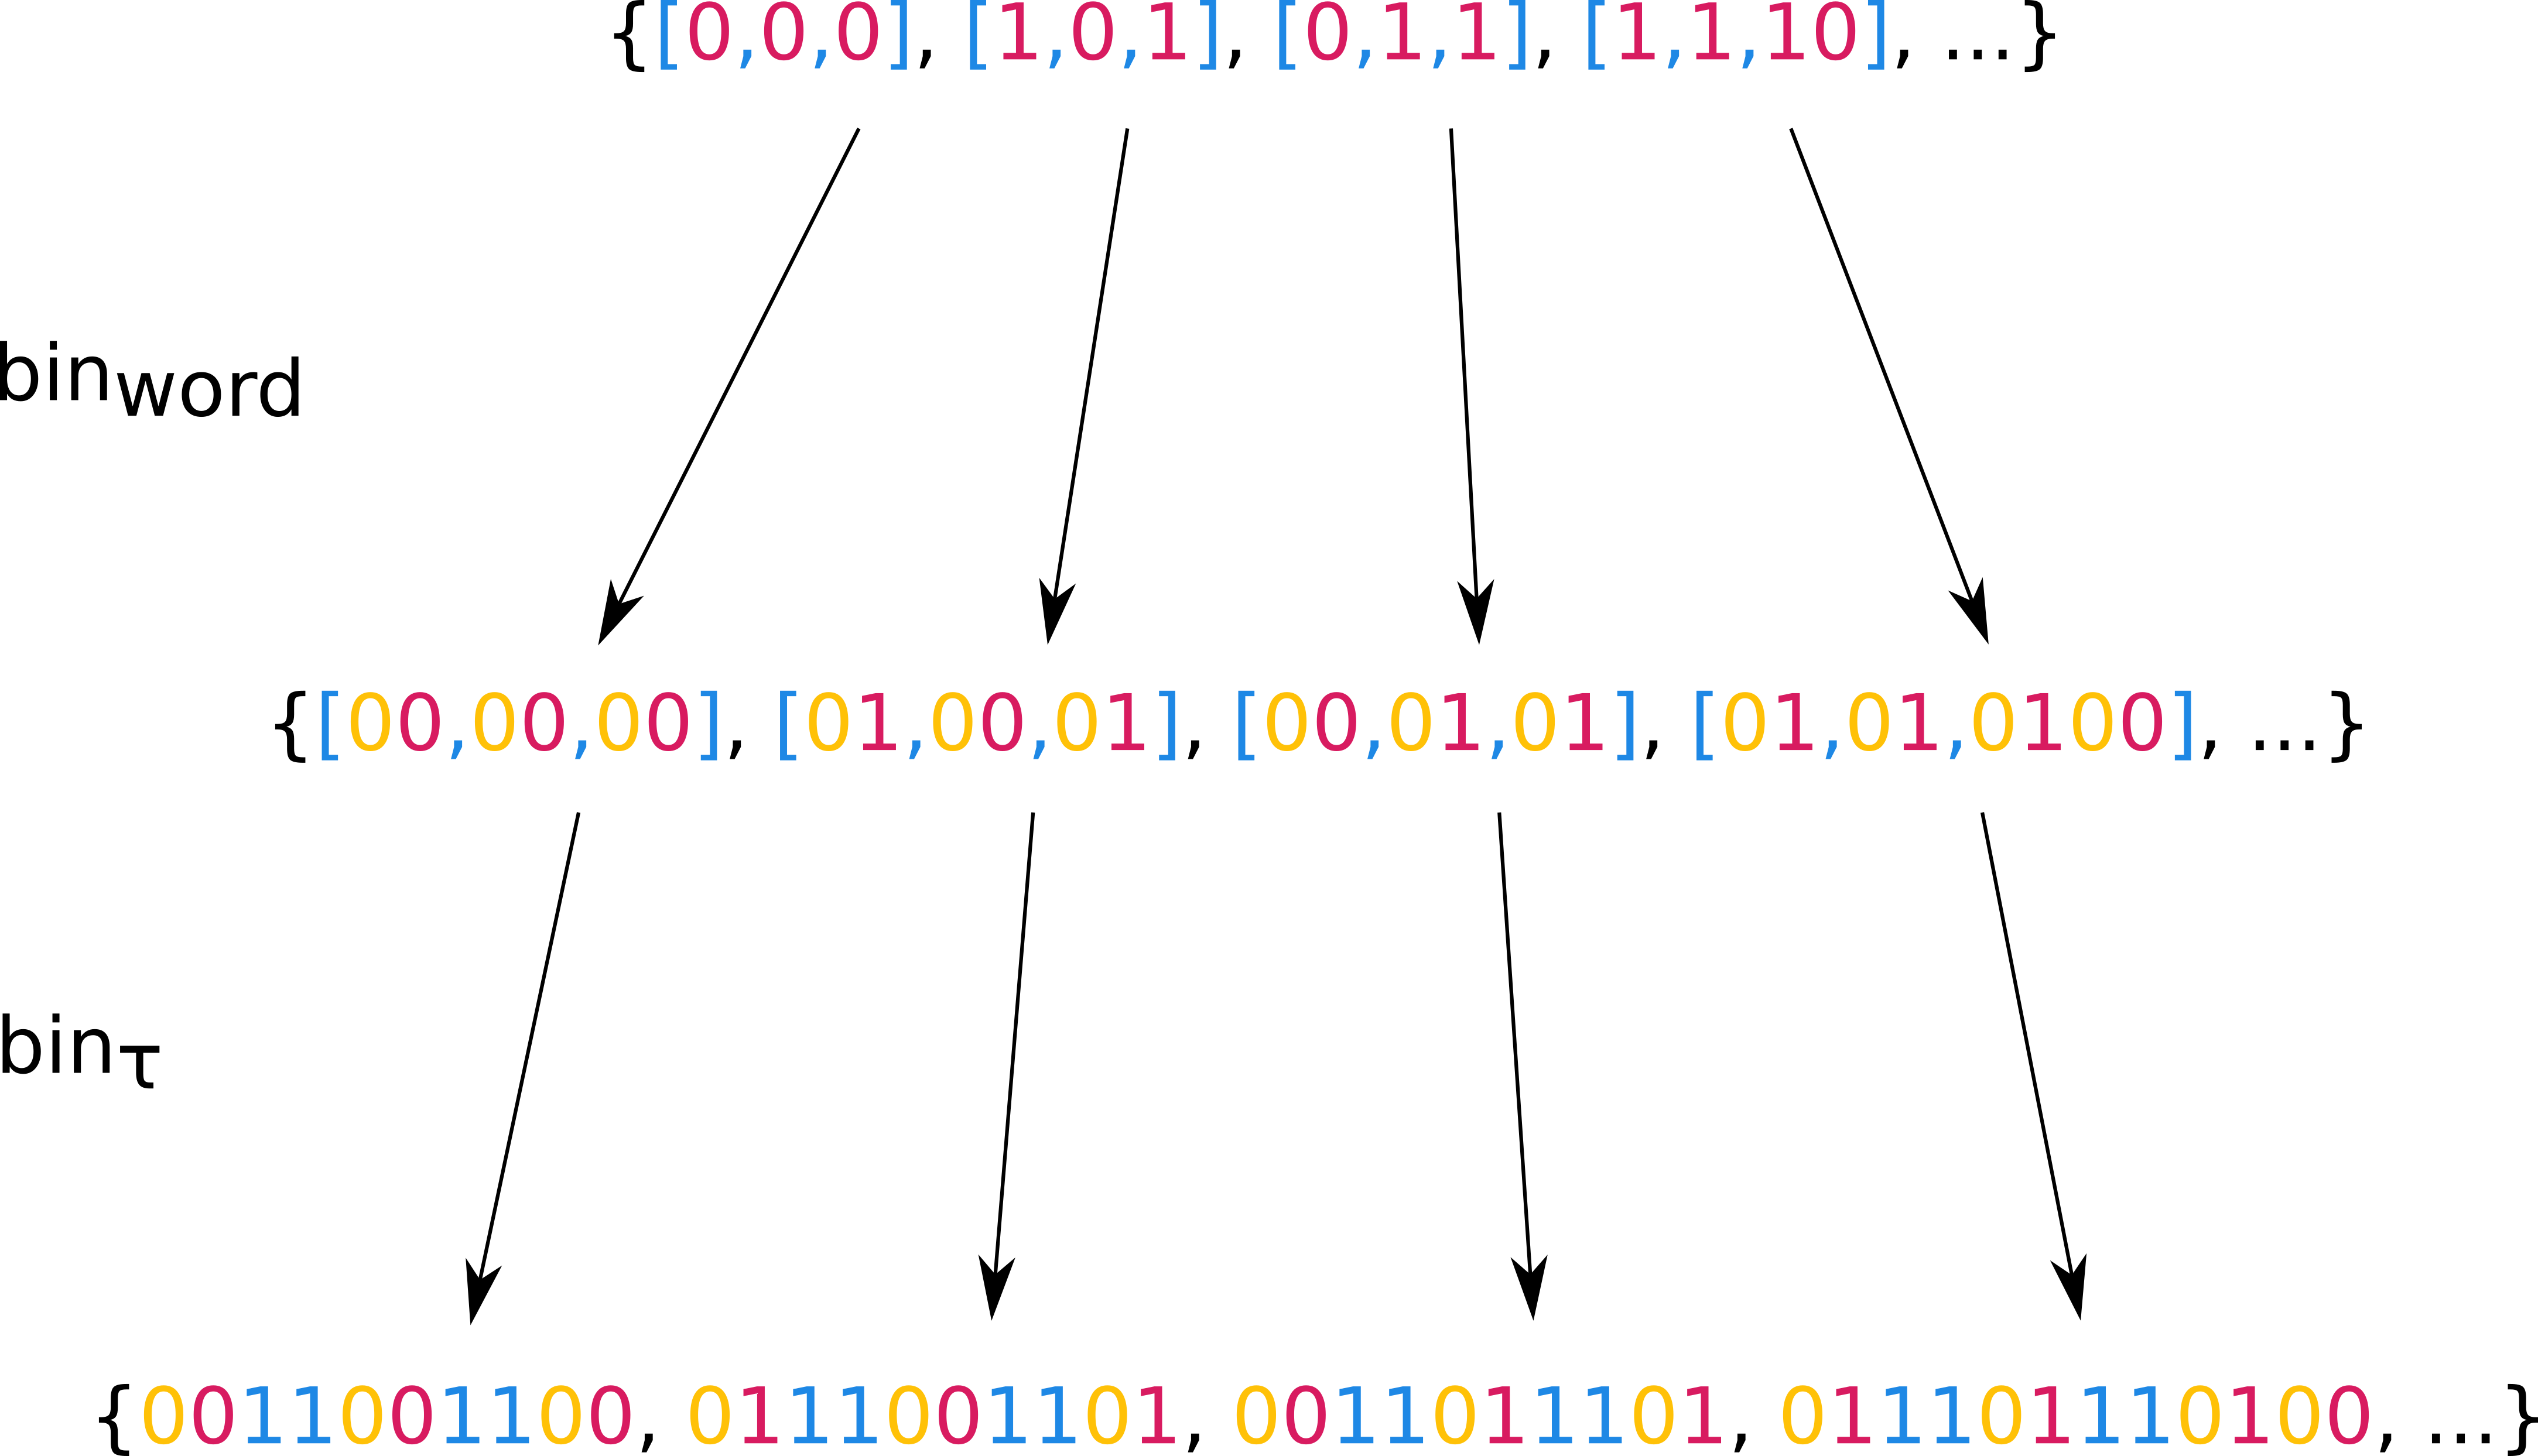
\includegraphics[width=\linewidth]{figures/fl.png}}
    \caption{Beispielhafte Repräsentation einer Funktion in einer formalen Sprache}\label{fig:fl}
\end{figure}

Z.B. ist $bin_{\mathcal{T}}([1,1,0]) = 0111011100$.
Da die Zeichenfolge 11 nicht Element der Wertemenge von $bin_{word}$ ist,
können wir so die Grenze der Binärwörter (die Kommata) im Tupel kodieren.
Damit haben wir eine generische Kodierung einer beliebigen Funktion
über $\Sigma = \{0,1\}$ angegeben.

Nach dieser Kodierung wäre also
\[
    L_{EVEN}^{'} = \{001101, 011100, 01001101, 01011100, \ldots \}
\]
und
\[
    L_{SUM} = \{0011001100, 0111001101, 011101110100, \ldots \}
\]

Somit haben wir eine Methode angegeben,
wie wir eine beliebige Funktion
(eine Menge von rechtseindeutigen, gleichlangen Tupeln)
als formale Sprache repräsentieren können,
deren Alphabet nur zwei Zeichen hat.


\subsection{Warum formale Sprachen?}\label{subsec:warumFormaleSprachen}

Sind Probleme also mit formalen Sprachen identisch?
Die Antwort darauf ist ein klares Nein.
Dass wir im vorigen Abschnitt \emph{zwei} Sprachen
$L_{EVEN}$ und $L_{EVEN}^{'}$ für \emph{ein} Problem gefunden haben,
zeigt, dass wir die beiden Entitäten nicht gleichsetzen dürfen:
Die Übersetzung eines Problems, das informell angegeben ist,
in eine formale Sprache ist nicht eindeutig.\footnote{
Das philosophische Problem, ob eine ``interessante'' Übersetzung jemals eindeutig sein kann,
wird auch in \cite{quine} und der Folgeliteratur besprochen.}

Zudem muss man ein Problem nicht in einer Sprache über einem binären Alphabet
$\Sigma = \{0,1\}$ kodieren,
wie wir es im vorangegangenen Abschnitt exemplarisch getan haben.
Man hätte auch Probleme mit einem unären, ternären
oder anderen Alphabet repräsentieren können.\footnote{
    Interessierte Leser:innen kommen in \cite{knuth2}, Chapter 4 (194-213) auf ihre Kosten.
}
Das obige Beispiel ist mit dem binären Alphabet im wahrsten Sinne des Wortes durchbuchstabiert,
weil es unseren Gewohnheiten entspricht
- deswegen nennen wir es \emph{kanonisch}.
Mit dem Begriff ``kanonisch'' weisen wir
auf eine quasi allgegenwärtige und akzeptierte Konvention hin,
ohne zu behaupten, die implizierte Wahl sei zwingend notwendig.
Unter welchen Umständen es einen Unterschied macht,
welche spezifische Sprache man als Repräsentation für ein Problem wählt,
ist eine Frage,
die wir in diesem Skript noch diskutieren wollen.

%Wir halten fest:
%In der theoretischen Informatik nutzen wir formale Sprachen,
%um Probleme zu repräsentieren,
%aber formale Sprachen und Probleme sind so wenig identisch,
%wie ein ausgestreckter Zeigefinger mit der Zahl 1 identisch ist.
%Der Zeigefinger \emph{kann} für die Zahl 1 stehen,
%aber er hat offensichtlich Eigenschaften,
%die die Zahl 1 nicht hat
%(diese ist nicht typischerweise neben einem Daumen zu finden).

Warum nutzen wir aber überhaupt formale Sprachen,
um Probleme zu formalisieren?
Formale Sprachen,
wie wir sie im vorangegangenen Abschnitt kennengelernt haben,
scheinen für praktische Anwendungen ungeeignet:
Sie wirken für Menschen sperrig und kompliziert,
im gegeben/gesucht-Format sind Probleme für die meisten Menschen schneller verständlich.

Es gibt aber einige Gründe,
die Repräsentation als formale Sprachen
für die Fragestellung der theoretischen Informatik zu nutzen:
\begin{itemize}
    \item Formale Sprachen sind konzise, unmissverständliche Beschreibungen von Problemen,
        die prinzipiell von jeder Maschine verarbeitet werden können,
        ohne dass wir uns auf eine bestimmte Hardware-Architektur oder Programmiersprache
        festlegen müssen.
    \item Formale Sprachen sind Mengen, daher können wir die Operationen der Mengenlehre
        auf sie anwenden.
        Z.B. kann man das Teilmengenverhältnis nutzen,
        um den Zusammenhang zwischen Problemen zu charakterisieren.
        Damit haben wir ein mächtiges Werkzeug zur Hand,
        den ``Raum'' der Probleme zu behandeln.
    \item Formale Sprachen haben Worte als Elemente und Zeichen als Teile der Worte.
        Dies erlaubt uns Zusammenhänge zwischen Problemen untersuchbar zu machen,
        indem wir einen Blick in die innere Struktur der Probleme werfen.
    \item Wir können All- und Existenzaussagen über Probleme als formale Sprachen formulieren
        und zum Teil beweisen.
    \item Aussagen über (effiziente) Berechenbarkeit werden mit den Methoden der Mathematik
        beweisbar, da wir u.a. die Ergebnisse der Mengenlehre, der Arithmetik
        und der Analysis anwenden können.
\end{itemize}

Die theoretische Informatik untersucht formale Sprachen auch als eigenen Gegenstand,
unabhängig davon, dass man formale Sprachen als formale Repräsentation von Problemen
interpretieren kann.
In unserem Skript konzentieren wir uns auf die Rolle von formalen Sprachen als
Repräsentation von Problemen,
in \autoref{ch:theorie} werden wir Hinweise durchgehen,
wie man das Studium der formalen Sprachen vertiefen kann.

\section*{Kapitelabschluss}
\subsection*{Zusammenfassung}
\begin{itemize}
    \item Erfahrene und kompetente IT-Fachkräfte erfassen den logischen Kern
        von IT-Alltagsaufgaben und können ihre Aufgaben daher effizient erledigen.
    \item Den logischen Kern können wir im gegeben/gesucht-Format fassen
        und so als Funktion verstehen. Diese Auffassung von Problemen nennen wir informell.
    \item Probleme lassen sich (aber auch) als formale Sprachen repräsentieren.
    \item Vorteil von formalen Sprachen ist, dass sie sich mit den Methoden der theoretischen Informatik
        bearbeiten lassen.
\end{itemize}
\subsection*{Aufgaben}
\begin{enumerate}
    \item Sei $I_{PLAYTASK}$: Gegeben: Eine Zahl $x \in \mathbb{N} < 4$ - Gesucht: $x + 1$.\\
        Kodieren Sie $I_{PLAYTASK}$ in eine formale Sprache über $\Sigma = \{0,1\}$.
    \item Geben sie ein Merkmal an, in dem sich \textbf{PLAYTASK} von allen Problemen
        in diesem Kapitel unterscheidet.
\end{enumerate}
